\documentclass[15pt]{article}
\usepackage[T1]{fontenc}
\usepackage[utf8]{inputenc}
\usepackage[polish]{babel}
\usepackage{indentfirst}
\usepackage{xcolor}
\usepackage{graphicx} 
\usepackage{subcaption}

\usepackage{fancyhdr}
\usepackage{lastpage}

\pagestyle{fancy}
\fancyhf[HR]{}

\AtBeginDocument{%
  \addtocontents{toc}{\protect\thispagestyle{empty}}%
  \addtocontents{lof}{\protect\thispagestyle{empty}}%
}

\cfoot{Strona \thepage \hspace{1pt} z \pageref{LastPage}}

\author{Mateusz Milewski}
\title{\textbf{Specyfikacja funkcjonalna}}
\frenchspacing
\begin{document}
\maketitle
\tableofcontents
\clearpage
\section{Opis ogólny}
\subsection{Nazwa programu}
Aplikacja będzie się nazywać ,,JapanApp''
\subsection{Poruszany problem}
Aplikacja jest tworzona w celach edukacyjnych, w ramach przedmiotu ,,Projekt Indywidualny'' na wydziale Elektrycznym Politechniki Warszawskiej. Aplikacja będzie aplikacją edukacyjną, której celem jest nauka alfabetu japońskiego. Jezyk japoński posiada pieć różnych systemów znakowych. Umiejętność czytania i pisania w trzech z nich(hiragana, katakana, kanji) jest kamieniem milowym do daleszej nauki tego języka. Z tego powodu aplikacja będzie miała na celu w łatwy i przystępny sposób uczyć tych trzech systemów znakowych.
\subsection{Użytkownik docelowy} 
Docelowym użytkownikiem będzie osoba prowadząca przedmiot ,, Projekt Indywidualny'', czyli opiekun projektu. Oprócz opiekuna projektu użytkownikiem może być zarówno młodzież, jak i dorośli, którzy szukają sposóbu na szybki i niezobowiązujący sposób na naukę języka japońskiego. 



\section{Opis funkcjonalności}
\subsection{Opis funkcjonalności}
Aplikcja ,, JapanApp'' skupiać się będzie na dwóch kluczowych aspektach, które są wymagane od osoby znającej dany system znakowy: umiejętność rozpoznawania znaków oraz umiejętność pisania znaków. Z tego powodu aplikacja będzie oferowała dwa tryby nauki:

\begin{itemize}
\item Pierwszy tryb będzie nosił nazwę ,,GuessIt''. Polegać on będzie na wyświetlaniu jednego ze znaków alfabetu japońskiego oraz czterech możliwych odpowiedzi, z których tylko jedna będzie poprawna. Użytkownik za wskaznia poprawnej odpowiedzi będzie otrzymywał punkty, a za zaznaczenie niepoprawnej odpowiedzi punkty będą odejmowane. Taki schemat będzie powtarzał się w cyklu trwającym 20 znaków. Na sam koniec pojawiać sie będzie ekran z liczbą zdobytych punktów. 
\item Drugi tryb będzie nazywał się ,,DrawIt''. Ten z kolej opierać się będzie na treningu pisania znaków. Na ekranie wyświetlać się będzie nazwa znaku z alfabetu oraz pole do rysowania palcem po ekranie. Zadaniem użytkownika będzie narysowanie za pomocą palca odpowiedniego znaku. Po zatwierdzeniu rysunku wyświetlany będzie ekran zarówno, z poprawnym wyglądem znaku, jak i tym narysowanym przez użytkownika. W tej samej chwili użytkownik będzie mógł ocenić, czy jego znak jest dobrze narysowany czy nadal wymaga poprawy. Odpowiednio do zaznaczonej odpowiedzi ,,dobrze'' lub ,,źle'' będą przyznawane punkty. Cały ten schemat będzie działał również w cyklu po 20 znaków i kończyć się będzie ekranem z podsumowaniem.
\end{itemize}

\section{Pojecia i pola formularza}
\subsection{Słownik z pojęciami}
Podstawowe pojecia występujące w dokumentach o aplikacji:
\newline
,,Alfabet'' i ,,System znakowy'' będą wykorzystywane naprzemiennie w dokumentacji, ponieważ w Japonii rzadko stosuje się pojęcie ,,Alfabet'', a raczej używa się systemów znakowych.
\newline
\newline
\textbf{Użytkownik}-- osoba używająca aplikację.
\newline
\textbf{Hiragana}-- jeden z dwóch głównych systemów pisma sylabicznego w jezyku japońskim, pozwalający opisywać japońskie słowa.
\newline
\textbf{Katakana}-- jeden z dwóch głównych systemów pisma sylabicznego w jezyku japońskim. Ten z kolej pozwala opisywać nazwy obcego pochodzenia, zapożyczenia.
\newline
\textbf{Kanji}-- systemem pisma logograficznego w jezyku japońskim, pozwalającego opisywać całe słowa za pomocą pojedynczego znaku.
\newline
\textbf{Suuji}-- to system liczbowy dziesiętny, identyczny jak system arabski.
\newline
\textbf{Roomaji}-- ostatni z systemów będacy już samymi znakimi z alfabetu łacińskiego/rzymskiego.



\section{Scenariusz działania programu}
\subsection{Scenariusz ogólny}
\begin{enumerate}
\item Pobranie aplikacji z ,,Sklepu Play'' na systemie Android.
\item Zainstalowanie jej.
\item Uruchomienie aplikacji.
\item Wybranie odpowiedniego trybu nauki.
\item Rozgrywka.
\item Zakończenie rundy po 20 znakach.
\item Podsumowanie.
\item Powrót do głównego menu.
\item Zakończenie działania aplikacji.

\end{enumerate}
\newpage
\subsection{Scenariusz szczegółowy}
\begin{enumerate}
\item Pobranie aplikacji z ,,Sklepu Play'' na systemie Android.
\item Zainstalowanie jej.
\item Uruchomienie aplikacji.
\item Wyświetlenie okna z menu głównym.
\item Wybranie odpowiedniego trybu nauki.
\begin{enumerate}
  \item Wybranie opcji ,,DrawIt''.
  \item Wybranie opcji ,,GuessIt''.
\end{enumerate}
\item Wyświetlenie okna z wyborem odpowiedniego systemu znaków (hiranaga, katakana, kanji).
\begin{enumerate}
  \item Wybranie hiragany.
  \item Wybranie katakany.
  \item Wybranie kanji.
\end{enumerate}
\item Wyświtlenie okna odpowiedniego do wybranych wcześniej opcji.
\begin{enumerate}
  \item Okno z rysowaniem znaku (opcja ,,DrawIt'' i z odpowiednim sytemem znaków).
  \item Okno z zgadywaniem jaki to znak (opcja ,,GuessIt'' i z odpowiednim systemem znaków).
\end{enumerate}
\item Rogrywka zgodnie z wyświetlonym oknem. 
\item Zakończenie rozgrywki po 20 etapach.
\item Wyświetlenie okna z podsumowaniem punktów.
\item Powrót do menu głównego.
\item Zakończenie działania aplikacji.
\end{enumerate}
\newpage
\subsection{Graficzna reprezentacja ekranów}
\subsubsection{Okna z wyborem}
Po uruchomieniu aplikacji pierwszym oknem, które będzie zawsze wyświetlane na samym początku to okno z menu głównym.
W tym oknie użytkownik będzie mógł wybrać, w którym trybie chce się uczyć: ,,DrawIt'' lub ,,GuessIt'', oraz będzie posiadać możliwość przejścia do okna z informacjami od twórców (Credits).

\begin{figure}[h!]
  \centering
  \begin{subfigure}[b]{0.35\linewidth}
    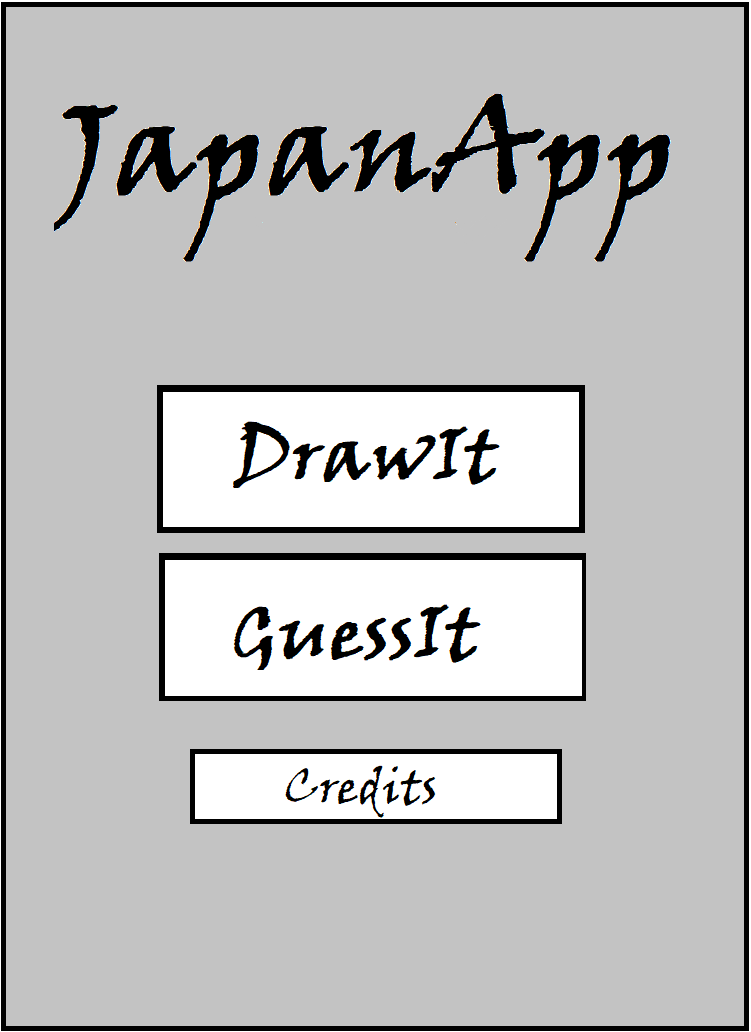
\includegraphics[width=\linewidth]{menu.png}
    \caption{Wizualizacja okna z menu głównym.}
  \end{subfigure}
  \begin{subfigure}[b]{0.35\linewidth}
    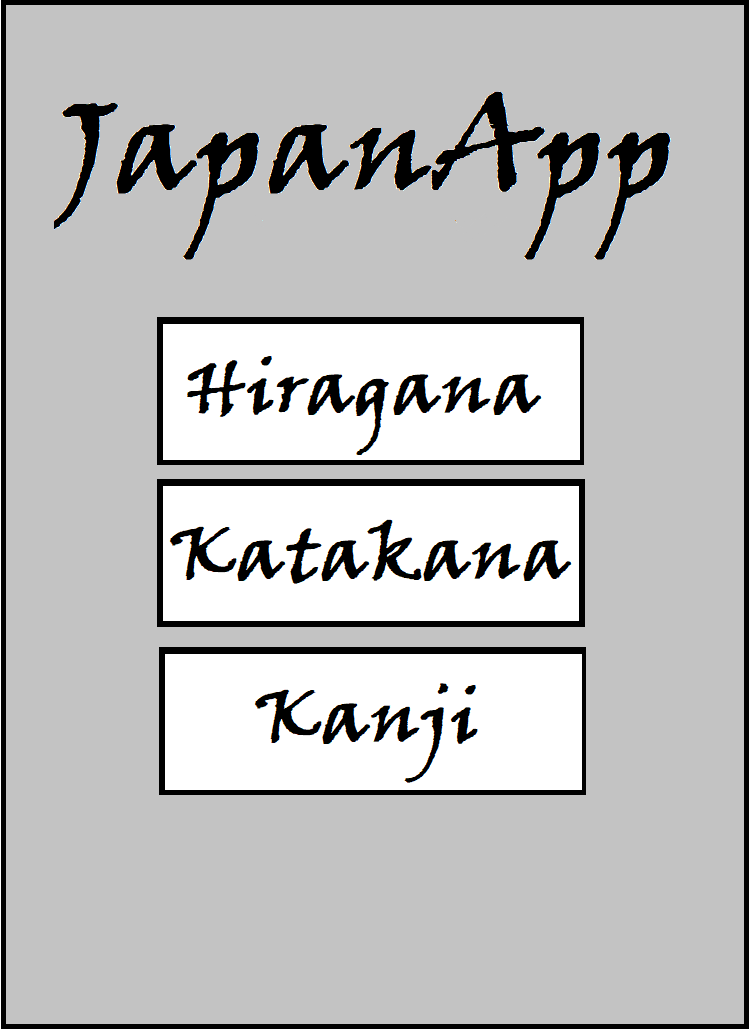
\includegraphics[width=\linewidth]{chose.png}
    \caption{Wizualizacja okna z wyborem systemu znakowego.}
  \end{subfigure}
  \label{fig:coffee}
\end{figure}

Po wybraniu któregokolwiek z dwóch trybów gry zostanie wyświetlone okno z wyborem systemu znakowego, którego aktualnie użytkownich chce się uczyć.
\subsubsection{Okna z rozgrywką}

Następnie po wybraniu sytemu znakowego wyświetlone zostanie okno z odpowiednim trybem ,,GuessIt'' lub ,,DrawIt''.
\begin{itemize}
\item W trybie ,,GuessIt'' zawarte będą trzy elementy:
    \begin{itemize}
      \item Nazwa systemu znakowego, którego użytkownik aktualnie się uczy.
      \item Duży obrazek z widocznym znakiem, który należy odgadnać.
      \item Cztery możliwe odpowiedzi, z których tylko jedna jest poprawna.
    \end{itemize}
\item W trybie ,,DrawIt'' będą już tylko dwa elementy:
\begin{itemize}
  \item Nazwa znaku, który należy narysować.
  \item Fragment ekranu, na którym użytkownik będzie mógł rysować.
\end{itemize}

  
\end{itemize}
\begin{figure}[h!]
  \centering
  \begin{subfigure}[b]{0.35\linewidth}
    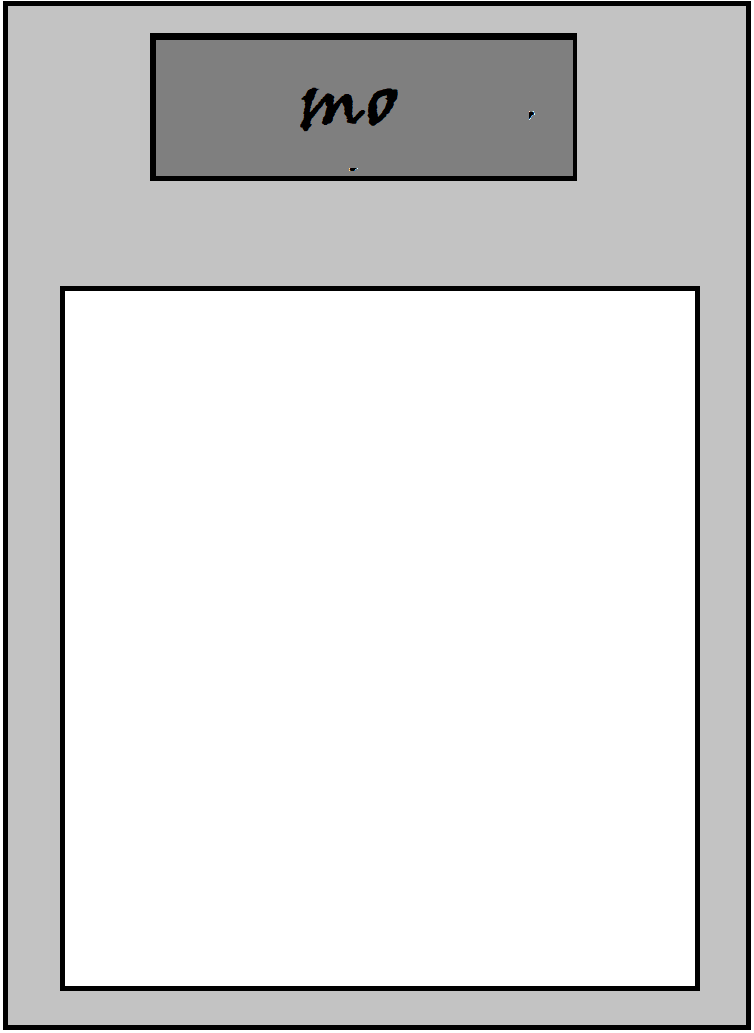
\includegraphics[width=\linewidth]{draw.png}
    \caption{Wizualizacja okna z trybem gry ,,DrawIt''}
  \end{subfigure}
  \begin{subfigure}[b]{0.35\linewidth}
    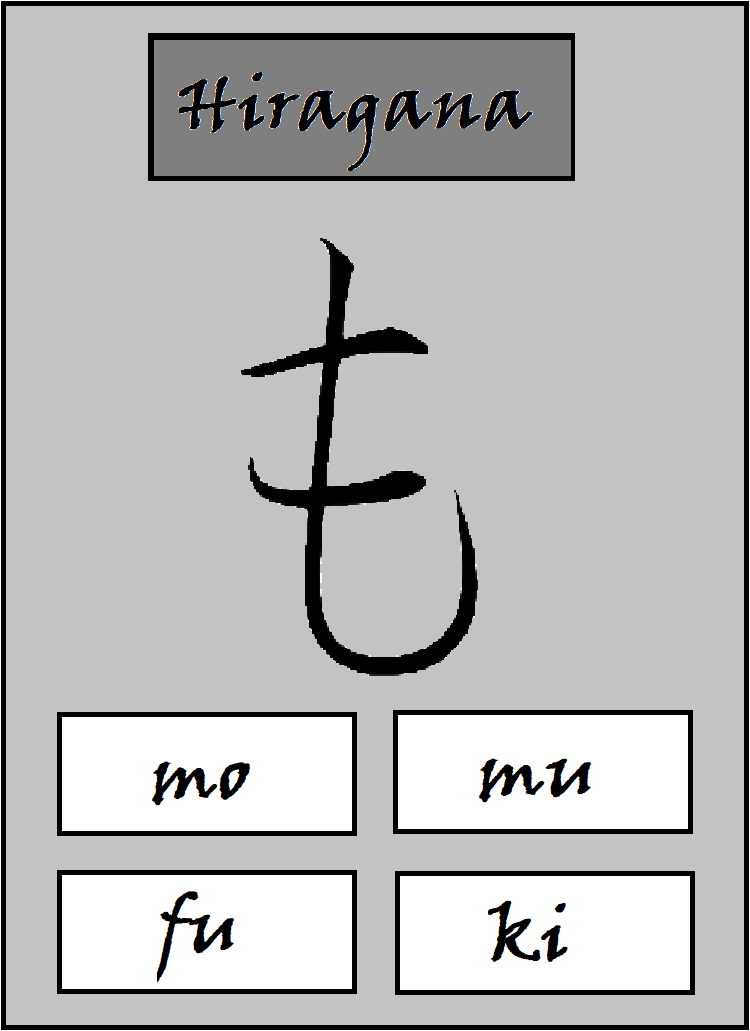
\includegraphics[width=\linewidth]{guess.png}
    \caption{Wizualizacja okna z trybem gry ,,GuessIt''}
  \end{subfigure}
  
  \label{fig:coffee}
\end{figure}

\subsubsection{Okna nieposiadające interakcji z użytkownikiem}
Po zakończeniu rozgrywki wyświetlone zostaje okno z podsumowaniem zdobytych punktów.
Ostatnim oknem, do którego użytkownik może wejść jest okno z informacjami od twórców. Bezpośrednie przejście do niego następuje poprzez kliknięcie w przycisk ,,Credits'' w menu głównym. Okno to będzie posiadać głównie informacje kto stworzył daną aplikację i w jakich celach.
\newline
\begin{figure}[h!]
  \centering
  \begin{subfigure}[b]{0.35\linewidth}
    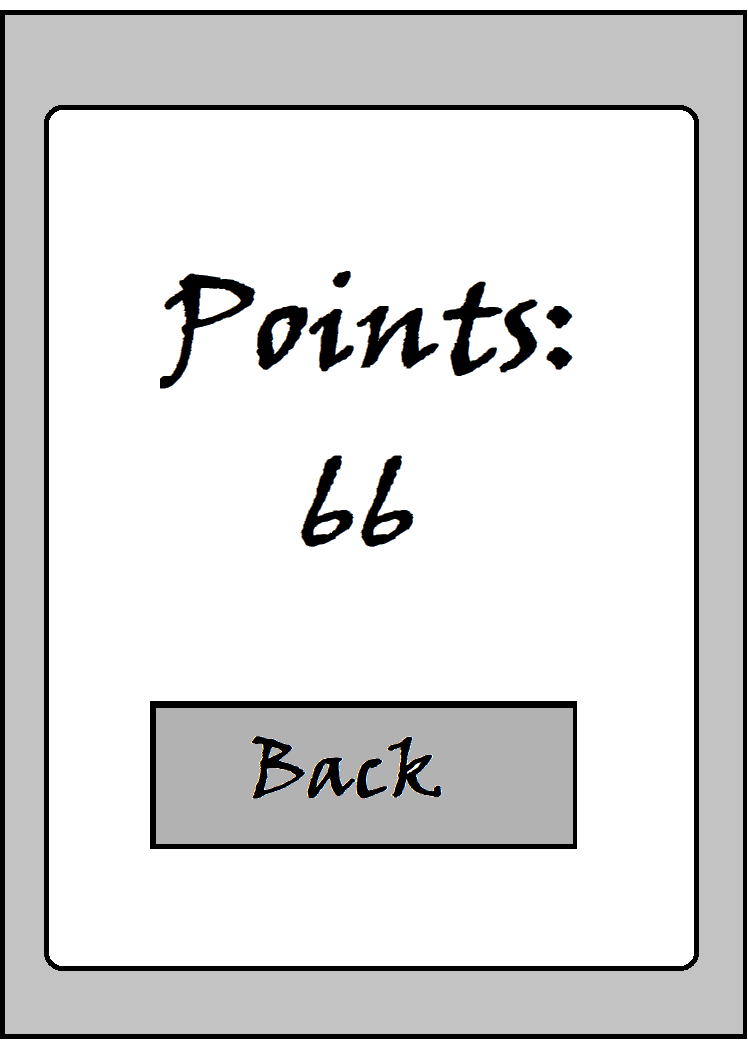
\includegraphics[width=\linewidth]{points.png}
    \caption{Wizualizacja okna z podsumowaniem}.
  \end{subfigure}
  \begin{subfigure}[b]{0.35\linewidth}
    
\includegraphics[width=\linewidth]{credits.png}
    \caption{Wizualizacja okna z informacjami od twórców.}
  \end{subfigure}
  \label{fig:coffee}
\end{figure}






\newpage
\section{Testowanie}
\subsection{Testowanie}
Poprawność działania aplikacji będzie testowania na kilku poziomach:
\begin{enumerate}
  \item Testowanie przy pomocy testów jednostkowych do kluczowych metod za pomocą biblioteki JUnit.
  \item Testowanie wydajności działania aplicji poprzez przeprowadzanie rozgrywek na różnych telefonach i w różnych trybach nauki.
\end{enumerate}

\end{document}